\newpage
\chapter{Similar-sized collisions: A parameter study}
\graphicspath{{./03figs/}}

A collision is cratering, when the impactor is much smaller than the target. In this case, the impactor hits the target completely and comes to a full stop, the result is a crater. Such a collision corresponds to a point source energy input into the target and can be treated like an explosion \citep{Melosh:2007p3502}. Scaling laws exist for the resulting crater depth and shape \citep{Holsapple:1993p3018}. 

In cratering collisions the impactor partly misses the target only for very grazing impact angles $\thimp \approx 90 \deg$ and the result deviates from pure cratering and becomes none-trivial. Such a case is shown in figure \label{ch03_fig03} on the right side where $\Rimp \ll \Rtar$. So a cratering collision results either in a complete hit or a complete miss. If on the other hand the target and the impactor are similar in size, this critical angle becomes much smaller than $90 \deg$ and the collision is called similar-sized, this is depicted on the left side of the figure in which case $\theta_{graz} \approx 45^\circ$. This grazing angle where roughly half of the impactor misses the target yields
\begin{equation}
\label{ch03_eq001}
\cos{ \theta_{graz} }= \frac{\Rtar}{\Rtar + \Rimp}
\end{equation}

\begin{figure}[htbp]
\begin{center}
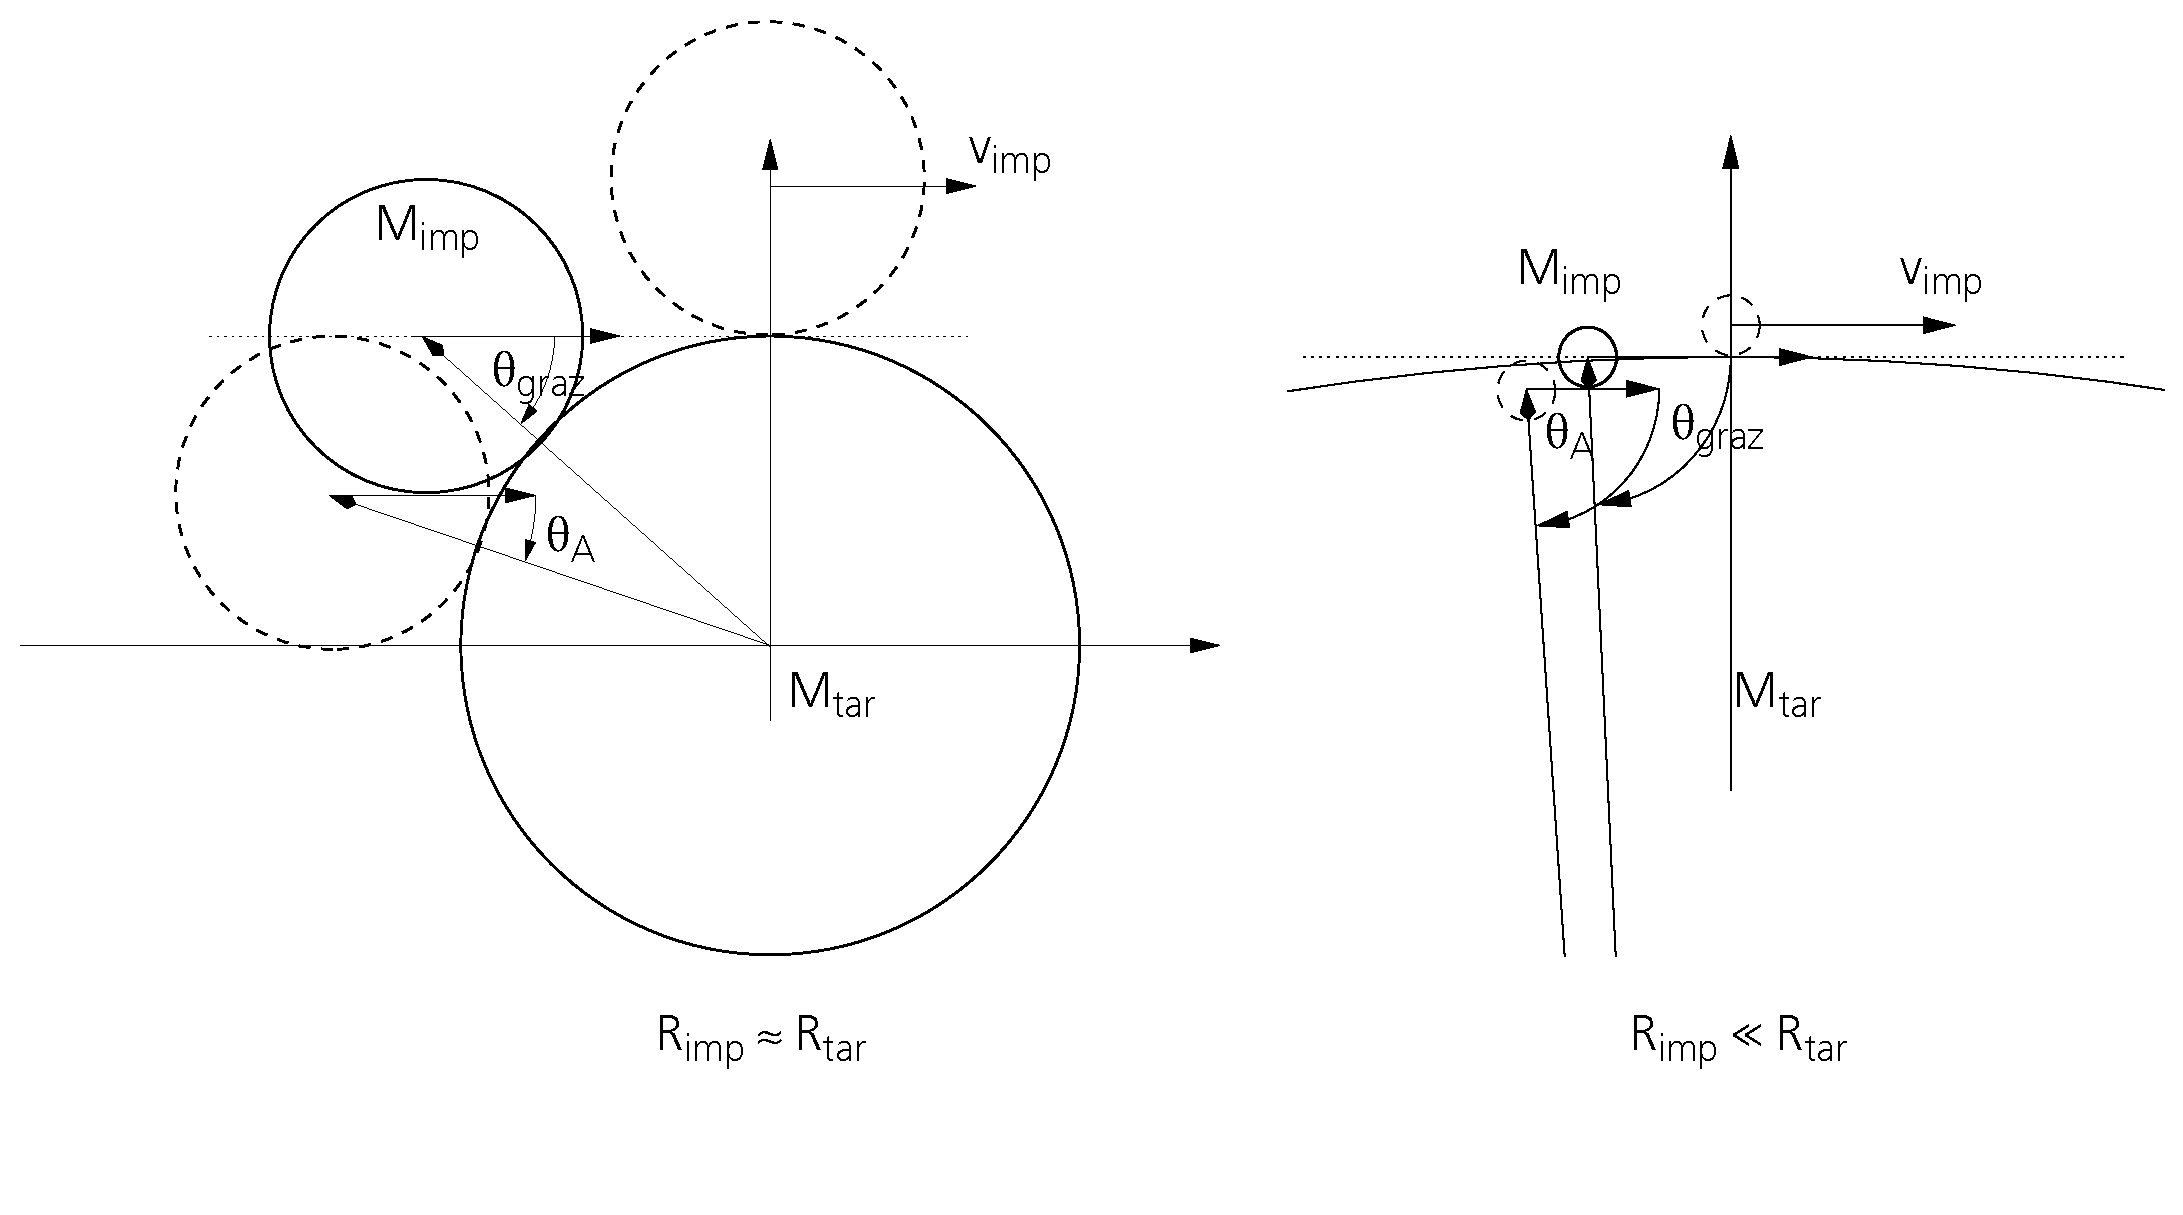
\includegraphics[scale=0.4]{03_grazing}
\caption{Impact geometry for a \SSC on the left side. The right plot shows a collision between a relatively small impactor compared to the target. The grazing impact angle $\theta_{graz}$ is defined as the angle for which half of the impactor simply grazes past the target \citep{Asphaug:2010p3539}. The dashed circles show the largest impact angle for which no impactor material would graze past the target $\theta_A$ and the $90^\circ$ impact angle for which the whole impactor grazes past the target.}
\label{ch03_fig03}
\end{center}
\end{figure}

\begin{figure}[htbp]
\begin{center}
\includegraphics[scale=0.7]{05_Mhit}
\caption{Relative volume of the impactor ($V_{hit, imp}$, left plots) and the target ($V_{hit, tar}$, right plots) hit by the other body as a function of impact angle (top plots) and impact parameter (bottom plots) for different mass ratios $\gamma$. Compare figure \ref{ch07_fig01} for an illustration of those volumes. Note that the ratio of radii scales with the cubic root of the mass ratio: $R_{imp} / R_{tar} \sim \sqrt[3]{\gamma}$. The dotted line shows for which impact angle half of the impactor volume grazes past the target. } 
\label{ch03_fig05}
\end{center}
\end{figure}

Assuming the impactor follows a straight trajectory, the volume missing the target can be calculated by integrating the cross section along the target volume (Compare appendix \ref{ch07_sec01} for the derivation). Figure \ref{ch03_fig05} on the left side shows the relative volume of the impactor missing the target ($V_{hit, imp}$) as a function of impact angle for different mass ratios $\gamma$ assuming constant and equal density spheres as bodies. The volume follows a step-function for very small impactors (small $\gamma$) with a sharp drop-off to zero near $90 \deg$. For similar-sized collisions with $\gamma = 0.1 \dots 1.0$ the relative volume smoothly increases for smaller impact angles opens the possibility for a variety of collisional outcomes between a total hit and a total miss. For example even for a rather small $\gamma = 0.1$, the relative volume hit by the impactor varies between 0 and 1 over an impact angle range of $30 \deg$.

Similar sized collisions are interesting, because bodies in planetary systems grow mainly by big accretionary events. Or in other words, the evolution of the largest bodies is dominated by similar-sized collisions. Many phenomena in planetary systems can best be explained as direct results of similar-sized collisions. Examples are the formation of the Earths Moon \citep{Benz:1985p1755}, Plutos companion Charon \cite{Canup:2005p1987} or also the anomalously high density of Mercury \cite{Benz:1988p3336}. Understanding similar-sized collisions is therefore key for understanding planet formation in general.

Compared to cratering collisions the interplay of the governing physics is more complex and there are only very basic scaling laws predicting the outcomes of similar-sized collisions. Hydrodynamics, gravity and thermodynamics interact in a interacted way and need to be simulated explicitly. The goal of this chapter is to perform a small parameter study in the regime of similar-sized collisions by performing a large number of impact simulations and then looking at various characteristic parameters describing the outcome of the collisions. The first section gives a quick overview of the physical processes involved in similar sized collisions and their associated timescales. In a second section, the detailed setup of the simulations and the used parameters are described. The actual results are presented in the third and discussed in the fourth section.

\section{Physics of similar-sized collisions}
Looking at the associated timescales of physics gives a feeling on what are the important aspect of physics in similar-sized collisions. In the gravity regime, where the impact velocities are in the order of the mutual escape velocity, similar-sized collisions possess the nice property scale-invariance on the first order: When the impact velocity is scaled to the escape velocity $\vesc$ and time to the collisional time $\tcol = ( \Rimp + \Rtar ) / \vesc$ the collision becomes self-similar. In other words: A collision at a given impact velocity and angle for a certain mass ration $\gamma = \Mimp / \Mtar$ has the same outcome for a target mass of $0.01 \ME$ and $1.0 \ME$ assuming the bodies have in both cases the same density and effects like shocks or compressibility can be neglected.

The collisional timescale is an estimate on how long it takes for the impactor to penetrate into the target and is given by
\begin{align}
\tau_{coll} = \frac{2 (\Rimp + \Rtar)}{\vimp} \sim \frac{\vesc}{\vimp} \frac{2 R_{tot}}{\vesc} \sim \frac{\vesc}{\vimp}  \frac{2 R_{tot}}{\sqrt{G \rho} R_{tot}} \sim \frac{\vesc}{\vimp} \frac{1}{\sqrt{\rho}}
\end{align}
where the mutual escape velocity is given by $\vesc = \sqrt{ 2 G \frac{\Mtar + \Mimp}{\Rtar + \Rimp} }$ and constant density bodies are assumed. Gravitational restitution happens on the gravitational timescale given by
\begin{align}
\tau_{grav} = \sqrt{\frac{3 \pi }{G \rho} } \sim \frac{1}{\sqrt{\rho}}
\end{align}
and is in the same order of magnitude as the collisional timescale. Both timescales depend on the bodies density. The collisional timescale also weakly depends on the mass ratio ($\sim \sqrt[3]{\gamma}$), but stays still in the same order of magnitude for the similar sized collisions mass ratios of $\gamma = 0.1 \dots 1$. For a collisions between with $\Mimp = \Mtar = 0.1\ME$ and $\Rimp = \Rtar = 0.55 \RE$ at their mutual escape velocity, the collisional timescale yields $50$ min, whilst the gravitational timescale for a mean-density of $4g/cm^3$ is around $100$ mins. Collisions for which the collisional timescale is on the same order of magnitude as the gravitational timescale is also called \emph{gravity dominated}, because the collision happens over a timescale in which gravity affects the whole system. If $\vimp \gg \vesc$, gravitational interacting during the collision process can be neglected and only plays a role for eventual re-accretion  of the remnants, although due to their high relative velocities the remnants will simply be dispersed.

Other physical effects are not scale-invariant, for example viscosity. \cite{Asphaug:2010p3539} argues as follows, that viscosity can be neglected in similar-sized collisions for bodies of at least a certain size: Characteristic stresses due to gravity are 
\begin{equation}
\sigma_{grav} \sim P_0 \sim G \rho^2 R^2
\end{equation}
where $P_0$ is the pressure inside the body with radius $R$. The strain rate $\dot{\epsilon}$ for a given Newtonian viscosity $\nu$ is then
\begin{equation}
\dot{\epsilon} = \frac{\sigma}{\nu}
\end{equation}
The strain which can develop over a gravitational timescale under viscosity is then
\begin{equation}
\epsilon = \frac{\dot{\epsilon}}{\tau_{grav}}
\end{equation}
Viscosity becomes an important effect, if the maximal strain which can develop over a gravitational timescale is only around unity. Or in other words, when the timescale for a strain of around unity becomes the same order of magnitude as the gravitational timescale, then viscosity is an important effect. Viscosity in the mantle of the early Earth was around $\nu \approx 10^9~\textrm{poise}$ \citep{2004Tectp.384...55W}, whereas for completely molten rock even lower values of around $\nu \approx 10^8~\textrm{poise}$ expected. \cite{Asphaug:2010p3539} gives a lower limit of a few $100km$ for solid and around $10km$ for partially molten bodies for which viscosity can be neglected and using a inviscid hydrodynamics solver is valid. Large bodies can be assumed to be molten during the early stages of planet formation 

Shocks are another effects where similar-sized collisions deviate from scale-invariance: The escape velocity scales $\vesc \sim M^\frac{1}{3}$ for constant density bodies \footnote{$\vesc = \sqrt[6]{8 \pi G^3 \rho} M^\frac{1}{3} \sim M^\frac{1}{3}$ for constant density sphere} and is around $1km/s$ for a density of $4g/cm^3$ and a mass of $10^{-3} \ME$. This is below the speed of sound in silicates ($\approx 3 km/s$, \cite{Melosh:2007p3502}), so that a collision with an impact velocity on the order of the escape velocity will produce acoustic waves but no strong shocks. For bodies with masses higher than a few Moon masses, the impact velocity comes into the same range as the speed of sound. Collisions now are in the hypervelocity regime and produce strong shock, leading to a considerable heating. 

The goal of this parameter study is now to get quantitative results for various quantities and to check whether they are scale-invariant or not.

\section{Setup and parameters used}
A similar-sized collisions encompasses many parameters, the most important ones being target mass $\Mtar$, mass ratio of the impact to the target $\gamma = \Mimp / \Mtar$, impact velocity $\vimp$ and impact angle $\thimp$. Often the scaled impact parameter $b'=\sin{\thimp}$ is alternatively used instead of the impact angle. These parameters span a 4-dimensional parameter space which will be explored in this parameter study. When using the impact angle, the four parameters have the nice property of having distinctive units, so we can write all four or a subset of them in the short form $\{\Mtar, \gamma, \thimp, \vimp\}$ with units $\{[g], [1], [\deg], [cm/s]\}$.

Additional parameters are the pre-impact rotation of both the impactor and the target, which in principle spans another 6-dimensions into the parameter space. Another parameter study concerning the formation of the Earths Moon by \cite{Canup:2008p3551} analyzed the effect of pre-impact rotation of the two bodies onto disk formation after the collision and found it to be non-negligible. The composition and interior thermal profiles of both bodies are also inform parameters. They both determine the density distribution inside the bodies and therefore also the dynamics of the collision. The internal profile furthermore determines the radius of the body and therefore the impact geometry, the mutual escape velocity and accordingly the actual impact velocity. These additional parameters are not further explored in this study.

\begin{figure}[htbp]
\begin{center}
\includegraphics[scale=0.7]{01_overview_params.pdf}
\caption{Overview of the sampling points in the 4-dimensional parameter space spanned by $\big\{ \Mtar, \gamma, \thimp, \vimp / \vesc \big\}$. The left plot shows the mass pairs for both bodies. Grey points denote \emph{r3} bodies (pure silicate), red points \emph{c1} bodies (chondritic, differentiated) and blue points \emph{i1} bodies (icy, differentiated). For each mass pair a total of 105 simulations sample the $\big\{ \thimp, \vimp / \vesc \big\}$ sub-space. Points in this sub-space are chosen so that regions of interest are sampled more accurately, for example in case of slow impact velocities ($\vimp < 1.5 \vesc$) and grazing impact angles ($\thimp > 45 \deg$).}
\label{ch03_fig01}
\end{center}
\end{figure}
\begin{figure}[htbp]
\begin{center}
\includegraphics[scale=0.8]{07_strucs.pdf}
\caption{Isentropic internal structures of the bodies used in the simulations. The first row of plots shows the density profiles, the second row the pressure and the third row the temperatures. The first column of plots shows silicate bodies with a $100 wt\%$ $\silc$ composition with the following masses from left to right: 0.1 (blue curve), 0.2 (red), 0.5 $\ME$ (magenta). The second column shows structures of differentiated bodies of chondritic composition with a $70 wt\%$ $\silc$ mantle and a $30 wt\%$ iron core: 0.002 (red), 0.007 (green), 0.01 (blue), 0.02 (red), 0.035 (black), 0.07 (green), 0.1 (blue), 0.2 (red), 0.7 (green) and 1.0 $\ME$ (blue). The last column on the right shows a few structures with a composition typical to regions beyond the snow line with $50 wt\%$ water ice, $35 wt\%$ $\silc$ and $15 wt\%$ iron. Masses range from 0.002 (red), 0.01 (blue), 0.02 (red), 0.1 (blue), 0.2 (red) and 1.0 $\ME$ (blue) from left to right. The radius of the structures depends on the average density and therefore also on the composition of the bodies. Icy bodies have low average densities compared to chondritic bodies. Note that the bodies entirely composed of $\silc$ have a higher average density than equally massive bodies with a chondritic composition, due to the higher compressibility of $\silc$ compared to iron. In the core of the pure silicate bodies, the density reached more than twice the reference density of $\silc$, while the iron cores of the chondritic bodies is only slightly compressed.}
\label{ch03_fig07}
\end{center}
\end{figure}

The strategy for sampling the parameter space goes as follows: For three different types of body composition sets of simulations are performed. Simulation set \emph{r3} uses homogeneous bodies made up of $100 \wtp~\silc$, simulation set \emph{c1} differentiated bodies with a chondritic composition of $70 \wtp~\silc$ and $30 \wtp~\iron$ and simulation set \emph{i1} uses differentiated bodies with a composition typical beyond the snow line of of $50 \wtp~\watr$, $35 \wtp~\silc$ and $15 \wtp~\iron$. Figure \ref{ch03_fig07} shows the internal structures for this three different types of bodies.

The general idea now is to use the \rss simulation with its simple internal structures to get a feeling for the different collisional effects and the scaling. The more realistic \css and \iss are then used to model actual collisions in planetary systems. Figure \ref{ch03_fig01} shows the sampling of the 4-dimensional parameter space mentioned above for the three different simulation sets.  The \rss simulation set uses three different mass ratios $\gamma = \Mimp / \Mtar$ with an impactor mass of $0.1 \ME$. The simulation sets \css and \iss cover three magnitudes of target masses in the range important for late terrestrial planet formation ($0.01 \dots 1 \ME$). The \css simulation set covers each target mass with at least impactors with a mass ratio of $\gamma = 0.2$ and  $0.7$. For the $0.1 \ME$ target, additional impactos with a mass ratio of $\gamma = 0.35$ and $0.1$ are also used. The \iss simulation set only uses impactors with a mass ratio of $\gamma = 0.2$. Figures \ref{ch03_fig29a} to \ref{ch03_fig29c} show the parameters used for each body pair in each simulation set. The number of particles is around $100'000$ in the target body, so that shocks can be resolved sufficiently well.

For each $\{ \Mtar, \Mimp \}$ combination, the parameter subspace spanned by $\big\{ \thimp, \vimp / \vesc \big\}$ is sampled. Figure \ref{ch03_fig01} shows on the right plot the used data points. The distribution covers areas of interest with more data points, for example for small impact velocities ($\vimp < 1.5 \vesc$) and grazing impact angles ($\thimp > 45 \deg$). In total a 105 individual simulations are performed for each body pair. The bodies used in the simulations are prepared as described in section \ref{ch02_sec04_ss02} and set up as described in\ref{ch02_sec04_ss04}. The initial separation $r_0$ is set to $5 (\Rimp + \Rtar)$ and simulations are integrated for $50 \tau_{coll}$. This is long enough in almost any case to get converging values for the interesting quantities in collisions. Figure \ref{ch03_fig31} shows various interesting quantities for the $\{0.1 \ME, 0.035 \ME, 1.60 \vesc, 38 \deg \}$ simulation in simulation set \css as a function of time. All of the quantities converge on a much smaller timescale than $50 \tau_{coll}$.
\begin{figure}[htbp]
\begin{center}
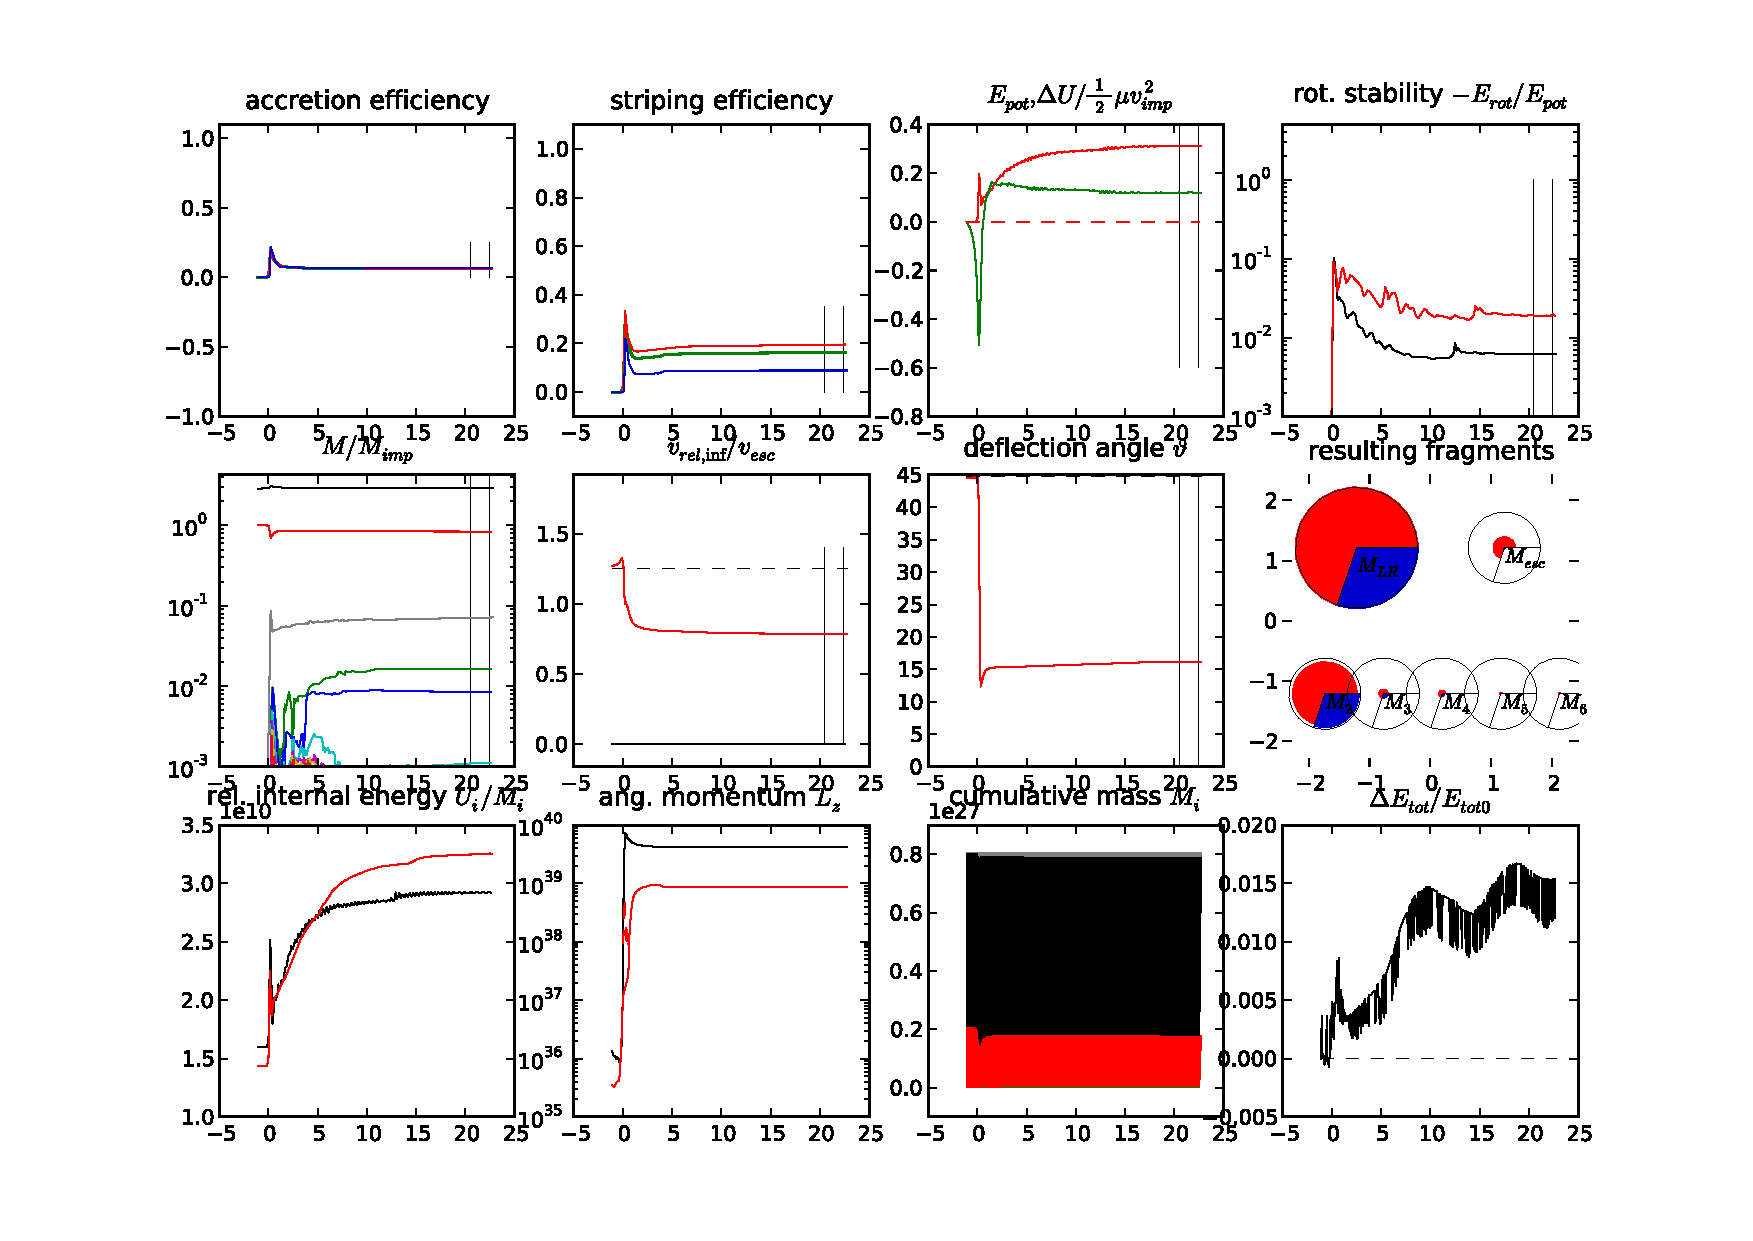
\includegraphics[scale=0.6]{31_sim_summary.pdf}
\caption{A summary for various quantities for the $\{0.1 \ME, 0.035 \ME, 1.60 \vesc, 38 \deg \}$ simulation in simulation set \css as a function of time. The x-axis in all plots denotes time in hours relative to the time of impact. One can see that all quantities converge much earlier than $50 \tau_{coll} = 22.76h$. The quantities shown in the top row are from left to right: Accretion efficiency $\xi$ (blue curve for iron, red for silicate and green for overall accretion), striping efficiency with the same color coding, change in potential (green) and internal energy (red) scaled to the reduced impact energy and finally on the far right the ratio of rotational to potential energy for the largest (black) and second remnant (red) as a measure for rotational stability. The middle row shows from the left: Remnant masses scaled to the impactor mass, relative velocity between the largest and the second remnant at infinity compared to the theoretical value expected from pure two-body interaction (dashed line), deflection angle of the second remnant compared to the theoretical two-body value (dashed line) and on the far right the composition of the remnant bodies and the ejecta. The bottom row shows from left to right: Mean specific internal energy ($erg/g$) for the largest (black) and the second remnant (red), angular momentum of the largest (black) and the second remnant (red) in $g~cm^2 / s$, mass partition into ejecta (grey), largest remnant (black), second remnant (red) and tertiary remnants (other colors). The far right shows the relative change in total energy over time as a measure for energy conservation. Errors in energy conservation mainly come from the removal of escaping particles at large distances. All the quantities will be explained below.}
\label{ch03_fig31}
\end{center}
\end{figure}
The only problematic cases where the quantities do not converge during this timescale, are when the impactor is being slowed enough to enter a closed orbit around the target with a very long orbital timescale. Such highly eccentric orbits lead to a secondary impact, where tidal effects can eject major fractions of the impactor out of the largest remnant. The orbital timescale may be $\gg 50 \tau_{coll}$, so that estimating the various quantities at that point in time leads to false results. In principle one could treat the secondary impact as a new collision scenario, but the problem is that our study does not cover impacts below the escape velocity and with impactor pre-rotation, which usually develops during the first collision. Such problematic cases occur for impact velocities slightly above the escape velocity and grazing impact angles. Figure \ref{ch03_fig30} shows such an example with the parameters $\{0.1 \ME, 0.1, 1.05 \vesc, 60 \deg \}$.
\begin{figure}[htbp]
\begin{center}
\includegraphics[scale=2.0]{30_elliptic_sim_out2.png}
\includegraphics[scale=2.0]{30_elliptic_sim_out3.png}
\includegraphics[scale=2.0]{30_elliptic_sim_out4.png}
\caption{Three successive snapshots along the impact plane of simulation $\{0.1 \ME, 0.01 \ME, 1.05 \vesc, 60 \deg \}$ of simulation set \css. The impactor (orange and light blue parts) is put on a highly eccentric orbit with an orbital time much longer than $50 \tau_{coll} = 30.43h$ (last snapshot).}
\label{ch03_fig30}
\end{center}
\end{figure}

The post-processing algorithms described in sections \ref{ch02_sec04_ss05} and \ref{ch02_sec04_ss07} are run every $0.1 \tau_{coll}$ in order to get continuous evolutions of the various quantities as shown in figure \ref{ch03_fig31}. A number of python scripts is used to run a simulation set from setting up the individual simulations, running them up to cleaning up the data and storing the results of the post-processing.

\afterpage{
%\clearpage% To flush out all floats, might not be what you want
\begin{landscape}
\begin{figure}[htbp]
\begin{center}
\includegraphics[scale=1.0]{29_params_r3.pdf}
\caption{Number of particles, mean density $\bar{\rho}$ and mean smoothing length $\bar{h}$ for the target and impactor bodies and $50 \tau_{coll}$ for a $\vimp = \vesc$ collision in the \rss simulation set.}
\label{ch03_fig29a}
\end{center}
\end{figure}
\begin{figure}[htbp]

\begin{center}
\includegraphics[scale=1.0]{29_params_c1.pdf}
\caption{Number of particles, mean density $\bar{\rho}$ and mean smoothing length $\bar{h}$ for the target and impactor bodies and $50 \tau_{coll}$ for a $\vimp = \vesc$ collision in the \css simulation set.}
\label{ch03_fig29b}
\end{center}
\end{figure}

\begin{figure}[htbp]
\begin{center}
\includegraphics[scale=1.0]{29_params_i1.pdf}
\caption{Number of particles, mean density $\bar{\rho}$ and mean smoothing length $\bar{h}$ for the target and impactor bodies and $50 \tau_{coll}$ for a $\vimp = \vesc$ collision in the \iss simulation set.}
\label{ch03_fig29c}
\end{center}
\end{figure}
\end{landscape}
}


\section{Results}
In this section we discuss several quantities which parametrize the outcome of simulated similar-sized collisions. Previous work is compared with the results of this parameter study and the differences are discussed. 
%%
% Largest remnant
%% 
\subsection{Largest remnant mass, accretion efficiency $\xi$, $\vcr$}
Maybe the most important quantity of a similar-sized collisions is the mass of the largest collision remnant $\Mlr$. It is the defined as the mass of the heaviest gravitationally bound system well after the collision. Note that this is not always just one body. Part of the largest remnant may also be satellites in stable orbits around the largest fragment. For example the Earth-Moon system is considered to be one single largest remnant of the giant impact. While most of the mass of the largest remnant naturally comes from the collision target, it can either accrete mass from the impactor or in high-energy events loose mass through erosion. A useful parameter related to $\Mlr$ is the accretion efficiency
\begin{equation}
\xi = \frac{\Mlr - \Mtar}{\Mimp}
\end{equation}
which gives us the change in mass from the target to the largest remnant normalized to the impactor mass $\Mimp$. If the impactor is accreted perfectly $\xi = 1$, if no mass is accreted or lost $\xi = 0$ and in case of target erosion where the target looses mass $\xi < 0$.

Figures \ref{ch03_fig08a} to \ref{ch03_fig08c} give the accretion efficiency for the three simulation sets as a function of the impact angle $\thimp$ for different impact velocities. For all three types of bodies and all mass ratios, the same characteristics can be observed: For very slow impact velocities of $\vimp = 1.00 \dots 1.05 \vesc$ (red and orange curves, x marker), the impactor is fully accreted independent of the impact angle. For very grazing impact angles a small fraction of the impactor is accelerated to an escaping velocity and escapes the remnant, so that the accretion efficiency is slightly below 1. This effect can be seen for $\thimp > 60 \deg$, especially for the $1.05 \vesc$ cases. A slight increase in impact velocity to $1.10 \vesc$ (green curve, x marker) lets the impactor miss the target almost unaltered if the impact angle is above a critical value, which seems to be mainly dependent on the mass ratio $\gamma$. Independent of type of body or the magnitude of the targets mass, this critical angle is between $60 \dots 75 \deg$ for $\gamma = 0.7$,  around $60 \deg$ for $\gamma = 0.2$ and slightly below $60 \deg$ for $\gamma = 0.1$. Above this critical angle, $\xi$ goes almost to 0. This is consistent with the results from \cite{Agnor:2004p3329} (compare figure 1) which finds a critical angle above $60 \deg$ for $\gamma = 1.0$. Additional simulations with $\gamma = 0.1$ and $0.5$ shown in figure 8 of \cite{Asphaug:2010p3539} also show critical impact angles for consistent with the results of this study (for a conversion between $\vinf$ and $\vimp$ check table \ref{ch03_tbl01}).
\begin{table}[htdp]
\begin{center}
\begin{tabular}{l|r|r|r|r|r|r|r|r}
$\vimp / \vesc$ & 1.00 & 1.05 & 1.10 & 1.15 & 1.20 & 1.30 & 1.40 & 1.50 \\
\hline
$\vinf / \vesc$ & 0.00 & 0.32 & 0.46 & 0.57 & 0.66 & 0.83 & 0.98 & 1.12\\
\hline
\hline
$\vimp / \vesc$ & 1.60 & 1.70 & 1.80 & 2.00 & 2.50 & 3.00 & 3.50 & 4.00\\
\hline
$\vinf / \vesc$ & 1.25 & 1.37 & 1.50 & 1.73 & 2.29 & 2.83 & 3.35 & 3.87\\
\end{tabular}
\end{center}
\caption{Conversion table $\vinf \leftrightarrow \vesc$}
\label{ch03_tbl01}
\end{table} 
Further increasing the impact velocity ($> 1.10 \vesc$) shifts this critical angle to smaller values and transforms the abrupt change from $\xi \approx 1$ to $\xi \approx 0$ into a smoother transition over a larger span of impact angle. For small mass ratios like $\gamma = 0.1$ in the \css or the simulation set or the $\gamma = 0.1$ and $0.2$ simulations in set \rss, the accretion efficiency follows a curve similar to the relative volume of the impactor hitting the target (black dashed line in all figures \ref{ch03_fig08a} to \ref{ch03_fig08c}). The impact velocity where the two quantities correlate best is between $1.20 \dots 1.40 \vesc$. The reason why this correlation gets weaker for higher mass ratios, is because the simple volumetric guess assumes that the target is not changed considerably and simply cuts through the impactor. The alteration of the target increases with higher mass ratios and model breaks down. Another complication is that equating the cross-section volume with the accreted mass only works for constant-density bodies. While this is roughly the case in simulation set \rss with its pure silicate bodies, this assumption breaks down in \css and \iss, where the heavier cores carry more kinetic energy per volume than the mantle material. In this case it makes a difference whether the core misses or hits the target. 

By further increasing the impact velocity, the accretion efficiency goes below $1$ even for $0 \deg$ head-on impacts. For high enough velocities it becomes negative so that the target is being eroded. While for hight impact velocities $\vesc > 3.00 \vesc$, the accretion efficiency becomes smaller for smaller impact angle, the effect reverses in an regime between $2.00 \dots 3.00 \vesc$, where the accretion efficiency actually increases again between for decreasing impact angles between $0 \dots 20 \deg$. This can be explained due to the fact that for a more head-on collision distributes the impact more evenly among the target, so that less mass reaches the required kinetic energy to leave the largest remnant. This effect is more prominent in the simulation sets with differentiated bodies (\css and \iss).

The results for the accretion efficiency are in agreement with previous work. \cite{Benz:1988p3336} performed SPH collision simulations with $\Mtar = 0.124 \ME$, $\gamma = 1/6$, $\vimp = 2.2 \dots 8.46 \vesc$ and $\thimp = 0 \dots 32 \deg$. Runs $9 \dots 11$ are comparable with simulations performed in this study here. While we have no data for $\Mtar = 0.124 \ME$ and $\gamma = 1/6$, the results should lie somewhere in between the runs for $\Mtar = 0.1 \ME$ and $\gamma = 0.1$ and $0.2$. Run 9 in  \cite{Benz:1988p3336} with $\{0 \deg, 3.34 \vesc \}$ obtained a $\gamma = -2.14$, in accordance with $\xi = -1.82$ for our simulation with $\{0.1 \ME, 0.1, 0 \deg, 3.50 \vesc \}$ and $\xi = -1.70$ for $\{0.1 \ME, 0.2, 0 \deg, 3.50 \vesc \}$. Run 10 with the parameters $\{ 0 \deg, 2.23 \vesc \}$ obtains $\xi = -0.14$ and lies in between $\xi = 0.48$ for out simulation $\{0.1 \ME, 0.2, 0 \deg, 2.50 \vesc \}$ and $\xi = -0.19$ for $\{0.1 \ME, 0.2, 0 \deg, 2.50 \vesc \}$. Run 11 uses a larger impcat angle with the parameters $\{ 32 \deg, 3.34 \vesc \}$ and yields $\xi = -1.12$, comparable with $\xi = -0.76$ of simulation $\{0.1 \ME, 0.1, 30 \deg, 3.50 \vesc \}$ and $\xi = -0.58$ of simulation $\{0.1 \ME, 0.2, 30 \deg, 3.50 \vesc \}$. The differences in the results between our simulations and  \cite{Benz:1988p3336}  are most probably due to the much lower resolution ($4k$ vs. $110k - 120k$ particles) and to the different version of ANEOS (dunite without molecules vs. $\silc$ with molecules).

\afterpage{
%\clearpage% To flush out all floats, might not be what you want
\begin{landscape}

\begin{figure}[htbp]
\begin{center}
\includegraphics[scale=1.0]{08_accreff_r3.pdf}
\caption{Accretion efficiency $\xi$ as a function of the impact angle for different relative impact velocities. Each subplot shows a set of simulations for a given target mass $\Mtar$ and mass ratio $\gamma = \Mimp / \Mtar$. Each point shows the outcome of an individual simulation of the \emph{r3} simulation set involving bodies composed purely of $\silc$. The black dashed line shows the relative volume of the impactor hitting the target for the given mass ratio (compare figure \ref{ch03_fig05}).}
\label{ch03_fig08a}
\end{center}
\end{figure}

\begin{figure}[htbp]
\begin{center}
\includegraphics[scale=1.0]{08_accreff_c1.pdf}
\caption{Accretion efficiency $\xi$ for the \emph{r3} simulation set with bodies of chondritic composition (compare figure \ref{ch03_fig08a}. Each row shows a different magnitude of target mass, each column a different mass ratio.}
\label{ch03_fig08b}
\end{center}
\end{figure}

\begin{figure}[htbp]
\begin{center}
\includegraphics[scale=1.0]{08_accreff_i1.pdf}
\caption{Accretion efficiency $\xi$ for the \emph{i1} simulation set with bodies of icy composition (compare figure \ref{ch03_fig08b}).}
\label{ch03_fig08c}
\end{center}
\end{figure}

\end{landscape}
}

Figures \ref{ch03_fig09a} to \ref{ch03_fig09c} show the accretion efficiency as a function of the impact velocity for different impact angles. All mass ratios in all simulation sets show the same characteristics: For grazing impact angles ($\thimp \gg \theta_{graz}$, compare figure \ref{ch03_fig03}), the accretion efficiency is a step function of the impact velocity. Either the impactor is almost perfectly accreted or misses the target completely. Target erosion is almost negligible, even for very high impact energies. For smaller impact angles then function then transitions towards a parabolic function. Escaping mass from the largest remnant is the proportional to the impact energy or the impact velocity squared. 

\cite{2010ApJ...714L..21K} performed a similar parameter study and extracted as a characteristic quantitiy the critical impact velocity
\begin{equation}
\xi(v_{cr}, \thimp, \Mtar, \Mimp) \doteq 0
\end{equation}
for which the accretion efficiency becomes zero as a function of impact angle, target and impactor mass. They performed SPH collision simulations with mass rations of $\gamma =$ 1.0, 0.66, 0.50, 0.33, 0.25, 0.17, 0.11 and $M_{tot} = \Mimp + \Mtar = 0.2 \dots 2.0 \ME$ at impact velocities between $\vimp = 1.0 \dots 3.0 \vesc$ at angles between $\thimp = 0 \dots 75 \deg$. Instead of the ANEOS equation of state used here, they used the Tillotson equation of state \cite{Melosh:1989p996} which does not include phase transitions for melting or vaporization. Both the target and the impactor are differentiated bodies with $70 \wtp~\silc$ and $30 \wtp~\iron$ as in our \css simulation set. They found the following empiric fitting function for
\begin{equation}
\label{ch03_eq002}
\vcr / \vimp = c_1 \Bigg( \frac{\Mtar - \Mimp}{\Mtar + \Mimp} \Bigg)^2 \big( 1 - \sin{\thimp} \big)^\frac{5}{2} + c_2 \Bigg( \frac{\Mtar - \Mimp}{\Mtar + \Mimp} \Bigg)^2 + c_3 \big( 1 - \sin{\thimp} \big)^\frac{5}{2}  + c_4
\end{equation}
with $c_1 = 2.43, c_2 = - 0.0408, c_3 = 1.86$ and $c_4 = 1.08$. The vertical lines in figure \ref{ch03_fig09a} to \ref{ch03_fig09c} show the predicted value for $\vcr$ for each mass ratio, target mass and impact angle. Our results in simulation set \css (\ref{ch03_fig09b}) match the predicted values quite well for $\thimp \ge 20 \deg$ and $\gamma \ge 0.2$. For $\thimp < 20 \deg$ equation \ref{ch03_eq002} predicts a strong increase in $\vcr$ for small decreases in impact angle, for example for $\gamma = 0.7$ $\vcr$ increase by over 50 \% from $\thimp = 15 \deg$ to $0 \deg$. Although our results also show a small increase in the impact velocity for which $\xi = 0$ for decreases in impact angle at already small values, it is not as large as in the empirical function from above. The main difference between the simulations presented here and the ones from \cite{2010ApJ...714L..21K} is the equation of state or particularly the lack of proper modeling of phase changes in the Tillotson equation of state. The amount of vaporization depends strongly on the impact regime. For gravity dominated collisions in the lunar mass regime ($\Mtar \approx 0.01 \ME$), only weak shocks and therefore no significant melting or vapor production is expected. With target masses in the order of the Earths mass, a significant amount of rock can be vaporized, due to impact velocities above the speed of sound of rock and the associated production of strong shocks. If the difference in the equation of state would be the cause of the disagreement of the critical velocities obtained from our results and the ones from the empiric law above, then our results should show a significant scale-dependence for the accretion efficiency. This is not the case. For a given mass range in a simulation set, the accretion efficiency is relatively scale-independent. The disagreement can best be explained by a  bad fit of equation \ref{ch03_eq002} with simulation results in general, probably also the ones from \cite{2010ApJ...714L..21K}. For very grazing angles equation \ref{ch03_eq002} predicts slightly too slow impact velocities, especially for small mass ratios. For instance at $\thimp = 45 \deg$ for $\{ \Mtar = 0.1 \ME, \gamma = 0.1\}$ the accretion efficiency yields $\xi \approx 0.8$ at the predicted critical impact velocity.

The simulation sets \iss and \rss with differently composed bodies show similar results for the critical velocity and therefore are also fit equation \ref{ch03_eq002} equally well as in the \css simulation set. \cite{2010ApJ...714L..21K} use equation \ref{ch03_eq002} to determine, whether collisions in terrestrial planet formation simulations are accreting or eroding mass on the target. Considering the disagreement between the fitting function and the simulation results suggest, that expression \ref{ch03_eq002} should not be used for $\thimp < 20 \deg$ and very high impact velocities, otherwise disruptive events while be falsely treated as accretionary.

\afterpage{
%\clearpage% To flush out all floats, might not be what you want
\begin{landscape}
\begin{figure}[htbp]
\begin{center}
\includegraphics[scale=1.0]{09_accreff_vimp_r3.pdf}
\caption{Accretion efficiency $\xi$ for the \emph{r3} simulation set as a function of impact velocity $\vimp$ for different impact angles. The vertical lines shows the predicted values from \cite{2010ApJ...714L..21K} for the critical impact velocity $v_{cr}$, where $\xi$ becomes negative and the target no longer accretes material but is eroded.}
\label{ch03_fig09a}
\end{center}
\end{figure}

\begin{figure}[htbp]
\begin{center}
\includegraphics[scale=1.0]{09_accreff_vimp_c1.pdf}
\caption{Accretion efficiency $\xi$ as a function of impact velocity $\vimp$ for different impact angles as in figure \ref{ch03_fig09a} for the \emph{c1} simulation set.}
\label{ch03_fig09b}
\end{center}
\end{figure}

\begin{figure}[htbp]
\begin{center}
\includegraphics[scale=1.0]{09_accreff_vimp_i1.pdf}
\caption{Accretion efficiency $\xi$ as a function of impact velocity $\vimp$ for different impact angles as in figure \ref{ch03_fig09a} for the \emph{i1} simulation set.}
\label{ch03_fig09c}
\end{center}
\end{figure}
\end{landscape}
}

\subsection{Catastrophic disruption threshold $Q^*_D$ and $Q^*_{RD}$}
Another quantity associated with the largest remnant is the specific impact energy required for catastrophic disruption, which is defined as a collision where the largest remnant is no more than half of the targets mass. The specific impact energy in its original defintion \cite{Benz1999Icar..142....5B} is the kinetic energy of the impactor 
\begin{equation}
Q = \frac{ \frac{1}{2} \vimp^2 \Mimp }{\Mtar} 
\end{equation}
The specific impact energy required for catastrophic disruption is denoted $Q^*_D$ and fulfills
\begin{equation}
\Mlr(Q^*_D) = 0.5 \Mtar
\end{equation}
More recent work \citep{Stewart:2009p3265, 2009ApJ...700L.118M, 2010ApJ...712L..73M, Leinhardt:2011p4060} considers the reduced mass and defines the specific reduced impact energy 
\begin{equation}
Q_R = \frac{ \frac{1}{2} \vimp^2 \mu }{\Mtar + \Mimp} \hspace{2.0cm} \mu = \frac{\Mtar \Mimp}{\Mtar + \Mimp} 
\end{equation}
and defines catastrophic disruption as a collision where the largest remnant has no more than half of the total mass $\Mtot = \Mtar + \Mimp$ with the reduced catastrophic disruption threshold $Q^*_{RD}$
\begin{equation}
\Mlr(Q^*_{RD}) = 0.5 \Mtot
\end{equation}
\cite{Stewart:2009p3265} propose the simple linear relationship between the largest remnant mass and $Q_R$
\begin{equation}
\label{ch03_eq003}
\Mlr / \Mtot = - 0.5 ( Q_R / Q^*_{RD} - 1 ) + 0.5
\end{equation}
$Q^*_{RD}$ is a constant depending on the material and scale-dependent physics. A velocity dependent form for this constant in \emph{cgs}-units is given by
\begin{equation}
Q^*_{RD} = \underbrace{ q_s R^{9\mu/(3-2\phi)}_{C1} \vimp^{2-3\mu} }_{\textrm{strength regime} } + \underbrace{ q_g R^{3 \mu}_{C1} \vimp^{2-3\mu}}_{\textrm{gravity regime}}
\end{equation}
where $R_{C1}$ is the radius of a body with mass $\Mtot$ and a density of $1 g/cm^3$. The first part comes from the required energy to overcome material strength, while the second part accounts for the gravitational binding energy. For small, solid bodies ($R < 1km$), the strength term is dominating, while it becomes negligible for large bodies ($R > 100km$). For the constants, \cite{Stewart:2009p3265} find the following constants for the basalt bodies in \cite{Benz1999Icar..142....5B}: $\mu = 0.5, \phi = 8, q_s = 7 \times 10^4, q_g = 10^{-4}$. In the gravity regime, \cite{2010ApJ...712L..73M} uses the same constant but changes $\mu = 0.4$. Obviously equation \ref{ch03_eq003} does not account for the collision geometry imposed by the impact angle and therefore deviations are expected. \cite{Stewart:2009p3265} state that the relationship \emph{does not hold for conditions that depart from the catastrophic disruption regime}. This excludes explicitly collisions which are merging ($\xi \approx 1$) or collisions in the super-catastrophic regime ($Q_R / Q^*_{RD} > 2$). Note also that the predicted $\Mlr / \Mtot$ is not scale invariant, as $Q^*_{RD}$ depends on the absolute velocity.

Figures \ref{ch03_fig15a} to \ref{ch03_fig15c} show the mass of the largest remnant relative to the total mass as a function of $Q_R / Q^*_{RD}$ for different impact angles. The dashed line shows the linear relationship \ref{ch03_eq003} which us supposed to match the results. As our simulations covered the same range of impact velocities for all mass ratios, the range of $Q_R$ covered is smaller for small mass ratios. For a small mass ratio, the impact velocity needs to be higher to reach the same value of $Q_R$ than for a collision with a larger mass ratio. As expected the value for $\Mlr / \Mtot$ does not match the linear relationship for collisions at the minimal specific impact energy $Q_{R,min} = \frac{ \frac{1}{2} \vesc^2 \mu}{\Mtot}$ which are perfectly accreting for all impact angles and therefore $\Mlr = \Mtot$. 

For larger values of $Q_R$ collisions become eroding and the relationship presents a reasonable fit for the determined largest remnant masses. The fit becomes better for small mass ratios. The concept of relating the largest remnant mass with the specific impact is based on the assumption, that the impact energy is perfectly coupled into the combined mass and can be used to overcome strength and the gravitational binding energy. But for impact angles above the grazing angle, considerable mass of the impactor misses the target and part of the impact energy can not be used erode the target. This effect can be seen in the results for simulations with impact angles near or above the grazing angle. For very head-on impact angles, the relationship surprisingly also shows a worse agreement, despite the fact that the impact energy is coupled perfectly into the combined mass. In all simulations, the $\Mlr / \Mtot$ decreases faster than linear for $\thimp < 20 \deg$. For small mass ratios ($\gamma = 0.35, 0.2, 0.1$), the impact angle for which the results match the prediction best is between $\thimp = 22 \dots 30 \deg$. For the larger mass ratios of $\gamma = 0.5$ and $0.7$, the slope of $\Mlr / \Mtot$ is best matched for $\thimp = 22 \deg$ for $Q_R > 0.5 Q^*_{RD}$ , but has quite a large offset. For smaller $Q_r$, small impact angles present a better match, but show a non-linear slope as for the small mass ratios. Nevertheless, the relationship \ref{ch03_eq003} predicts the largest remnant mass within a factor of 2 for all cases and much better for most eroding cases, which is in accordance with \cite{2009ApJ...700L.118M}. As the accretion efficiency $\xi$ above, the agreement of the relationship with the results is basically scale-invariant. The differences between different mass regimes show now systematic differences.

\afterpage{
%\clearpage% To flush out all floats, might not be what you want
\begin{landscape}
\begin{figure}[htbp]
\begin{center}
\includegraphics[scale=1.0]{15_QQRD_r3.pdf}
\caption{Scaled largest remnant masses $\Mlr / M_{tot}$ as a function of the relative specific impact energy $Q_R / Q^*_{RD}$ as defined in \cite{Stewart:2009p3265} and using the parameters for $Q^*_{RD}$ as in \cite{2010ApJ...712L..73M}. The coloured lines solid lines show the simulation values for the \emph{r3} simulation set and the dashed black line shows the predicted value from the scaling law.}
\label{ch03_fig15a}
\end{center}
\end{figure}

\begin{figure}[htbp]
\begin{center}
\includegraphics[scale=1.0]{15_QQRD_c1.pdf}
\caption{Scaled largest remnant masses $\Mlr / M_{tot}$ as a function of the relative specific impact energy $Q_R / Q^*_{RD}$ as in figure \ref{ch03_fig15a}, but for the \emph{c1} simulation set.}
\label{ch03_fig15b}
\end{center}
\end{figure}

\begin{figure}[htbp]
\begin{center}
\includegraphics[scale=1.0]{15_QQRD_i1.pdf}
\caption{Scaled largest remnant masses $\Mlr / M_{tot}$ as a function of the relative specific impact energy $Q_R / Q^*_{RD}$ as in figure \ref{ch03_fig15a}, but for the \emph{i1} simulation set.}
\label{ch03_fig15c}
\end{center}
\end{figure}
\end{landscape}
}


%%
% second remnant 
%% 
\subsection{Second remnant}

\cite{Agnor:2004p3329} compare with figure 2\\

mainly for next largest bodies\\
mantle striping\\
impactor perspective\\
accr. efficiencies for individual components \\
compositional changes for h\&r \\
introduce alternative impact angles $\theta_{core}$ \\
give volumetric estimate \\
compare sound speed with impact velocity to check for shocking (vimp vs. vsound), define vimprel which becomes supersonic \\

\begin{equation}
\delta_X = \frac{\Msr - M_{imp}}{M_{imp}} \Bigg|_{X}
\end{equation}


\afterpage{
%\clearpage% To flush out all floats, might not be what you want
\begin{landscape}
\begin{figure}[htbp]
\begin{center}
\includegraphics[scale=1.0]{26_SR_M_r3.pdf}
\caption{Second remnant mass $\Msr$ as a function of relative velocity at infinity before impact $\v_{-\infty} / \vesc$ for the \emph{r3} simulation set. Simulations with a second remnant below 5\% of the impactors mass are not shown.}
\label{ch03_fig26a}
\end{center}
\end{figure}

\begin{figure}[htbp]
\begin{center}
\includegraphics[scale=1.0]{26_SR_M_c1.pdf}
\caption{Second remnant mass $\Msr$ as a function of relative velocity at infinity before impact $\v_{-\infty} / \vesc$ as in figure \ref{ch03_fig26a} but for the \emph{c1} simulation set.}
\label{ch03_fig26b}
\end{center}
\end{figure}

\begin{figure}[htbp]
\begin{center}
\includegraphics[scale=1.0]{26_SR_M_i1.pdf}
\caption{Second remnant mass $\Msr$ as a function of relative velocity at infinity before impact $\v_{-\infty} / \vesc$ as in figure \ref{ch03_fig26a} but for the \emph{i1} simulation set.}
\label{ch03_fig26c}
\end{center}
\end{figure}
\end{landscape}
}

%%
% Tertiary remnants
%%
\subsection{Tertiary remnants}

\afterpage{
%\clearpage% To flush out all floats, might not be what you want
\begin{landscape}
\begin{figure}[htbp]
\begin{center}
\includegraphics[scale=1.0]{27_TR_M_r3.pdf}
\caption{Tertiary remnant masses $M_{TR} = \sum_{i=3}^N M_i$ as a function of impact angle for the \emph{r3} simulation set.}
\label{ch03_fig27a}
\end{center}
\end{figure}

\begin{figure}[htbp]
\begin{center}
\includegraphics[scale=1.0]{27_TR_M_c1.pdf}
\caption{Tertiary remnant masses $M_{TR} = \sum_{i=3}^N M_i$ as a function of impact angle for the \emph{c1} simulation set.}
\label{ch03_fig27b}
\end{center}
\end{figure}

\begin{figure}[htbp]
\begin{center}
\includegraphics[scale=1.0]{27_TR_M_i1.pdf}
\caption{Tertiary remnant masses $M_{TR} = \sum_{i=3}^N M_i$ as a function of impact angle for the \emph{i1} simulation set.}
\label{ch03_fig27c}
\end{center}
\end{figure}
\end{landscape}
}


%%
% ejecta 
%% 
\subsection{Ejecta}
% radiation transfer
Shocks in similar-sized collisions are another departure from 
\begin{align}
\tau_{cool} = \frac{c^2 \sigma}{ 2 \sigma_{SB} T^4}
\end{align}
\cite{Thompson:1988p3451}
radiation transfer: not important because of short timescales (everything in opaque thermal equilibrium): compare stefan boltzmann cooling power (Pahlevan?)
cite Lisse\\
analyze ejecta, entropy and energy of ejecta \\
show decay of shock wave plot\\ % TODOPLOT


\afterpage{
%\clearpage% To flush out all floats, might not be what you want
\begin{landscape}
\begin{figure}
\begin{center}
\includegraphics[scale=1.0]{20_ejecta_r3.pdf}
\caption{Mass averaged mean disk eccentricities for the largest remnant disk as a function of impact angle for different impact velocities in the \emph{r3} simulation set. Simulations with a largest remnant disk mass below $0.1\% M_tot$ are omitted.}
\label{ch03_fig20a}
\end{center}
\end{figure}

\begin{figure}
\begin{center}
\includegraphics[scale=1.0]{20_ejecta_c1.pdf}
\caption{Mass averaged mean disk eccentricities for the largest remnant disk as a function of impact angle for different impact velocities in the \emph{r3} simulation set. Simulations with a largest remnant disk mass below $0.1\% M_tot$ are omitted.}
\label{ch03_fig20b}
\end{center}
\end{figure}

\begin{figure}
\begin{center}
\includegraphics[scale=1.0]{20_ejecta_i1.pdf}
\caption{Mass averaged mean disk eccentricities for the largest remnant disk as a function of impact angle for different impact velocities in the \emph{r3} simulation set. Simulations with a largest remnant disk mass below $0.1\% M_tot$ are omitted.}
\label{ch03_fig20c}
\end{center}
\end{figure}
\end{landscape}





%%
% compositional changes
%% 
\subsection{Compositional changes}
compare with Marcus 2009, Benz 1988
changes to largest remnant (mantle striping): compare with Marcus 2009 (\cite{2009ApJ...700L.118M}) and 2010 (\cite{2010ApJ...712L..73M})

changes to second remnant (striping efficiency)

\afterpage{
%\clearpage% To flush out all floats, might not be what you want
\begin{landscape}
\begin{figure}[htbp]
\begin{center}
\includegraphics[scale=1.0]{18_strpeff_vimp_c1.pdf}
\caption{Difference of striping efficiency for silicate and iron ($\delta_{\silc} - \delta_{Fe}$) as a function of impact angle for the \emph{c1} simulation set.}
\label{ch03_fig18a}
\end{center}
\end{figure}

\begin{figure}[htbp]
\begin{center}
\includegraphics[scale=1.0]{18_strpeff_vimp_i1.pdf}
\caption{DIfference of striping efficiency for silicate and iron ($\delta_{\silc} - \delta_{Fe}$) and for water ice and silicate ($\delta_{H_2 O} - \delta_{\silc}$) as a function of impact angle for the \emph{i1} simulation set.}
\label{ch03_fig19a}
\end{center}
\end{figure}

\begin{figure}[htbp]
\begin{center}
\includegraphics[scale=1.0]{23_impa_vs_corea_c1.pdf}
\caption{The impact angle of the impactors iron core against the targets iron core $\theta_{Fe}$ as a function of actual impact angle $\thimp$ of the bodies for the \emph{c1} simulation set.}
\label{ch03_fig23a}
\end{center}
\end{figure}

\begin{figure}[htbp]
\begin{center}
\includegraphics[scale=1.0]{23_impa_vs_corea_i1.pdf}
\caption{The impact angle of the impactors iron core against the targets iron core $\theta_{Fe}$ and the silicate layers of the two bodies $\theta_{\silc}$ as a function of actual impact angle $\thimp$ of the bodies for the \emph{i1} simulation set.}
\label{ch03_fig23b}
\end{center}
\end{figure}

\begin{figure}[htbp]
\begin{center}
\includegraphics[scale=1.0]{34_compo_QQRD_c1.pdf}
\caption{The iron fraction of the largest remnant $M_{lr, Fe} / \Mlr$ as a function of the relative specific impact energy $Q_R / Q^*_{RD}$ for different impact angles in simulation set \css. The black dashed line shows the power law provided in \cite{2009ApJ...700L.118M}.}
\label{ch03_fig34}
\end{center}
\end{figure}
\end{landscape}
}


%%
% rotation stuff
%% 
\subsection{Spin-up, critical angular momentum}
\cite{Canup:2000p3542}: critical ang. momentum\\
critical T / W for largest remnant\\
critical T / W for second remnant at large $\thimp$ (get data)\\
how to get from Erot and I to a rotation rate:
\begin{equation}
T = 2 \pi \sqrt{ \frac{I}{2 E_{rot}} }
\end{equation}
shedding of material due to rotational ejection well before stability limits given in the literature. why? departure from solid body rotation.\\
$L_{bound}$ vs. $L_{imp}$ \\
$t = \frac{T}{|W|}$
$t_{crit} = 0.2738$ for McLaurin spheroids \citep{1987gady.book.....B} \citep{chandrasekhar1969ellipsoidal}


\afterpage{
%\clearpage% To flush out all floats, might not be what you want
\begin{landscape}
\begin{figure}[htbp]
\begin{center}
\includegraphics[scale=1.0]{19_rotperiod_r3.pdf}
\caption{Rotation period of the largest remnant as a function of impact angle for the \emph{r3} simulation set. Only particles in the remnant are considered which are part of the largest clump and not in a disk orbit. Solid body rotation is assumed for calculating the rotation period by simply comparing the rotational energy with the moment of intertia: $T = 2 \pi \frac{I}{2 E_{rot}}$.}
\label{ch03_fig19a}
\end{center}
\end{figure}

\begin{figure}[htbp]
\begin{center}
\includegraphics[scale=1.0]{10_rotstab_r3.pdf}
\caption{Dimensionless rotational stability parameter $t = \frac{T}{|W|}$ comparing the rotational energy $T$ with the potential energy $W$ for the largest remnant in the \emph{r3} simulation set. Note that again only particles from the actual clump are considered for calculating both energies. Disk particles are not considered.}
\label{ch03_fig10a}
\end{center}
\end{figure}

\begin{figure}[htbp]
\begin{center}
\includegraphics[scale=1.0]{25_LvsLimp_r3.pdf}
\caption{Angular momentum of the largest remnant perpendicular to the impact plane $[L_{LR}]_z$ relative to the impact angular momentum $L_{imp}$ as a function of impact angle for the \emph{r3} simulation set.}
\label{ch03_fig25a}
\end{center}
\end{figure}


\begin{figure}[htbp]
\begin{center}
\includegraphics[scale=1.0]{19_rotperiod_c1.pdf}
\caption{Rotation period of the largest remnant as a function of impact angle for the \emph{c1} simulation set as in figure \ref{ch03_fig19a} }
\label{ch03_fig19b}
\end{center}
\end{figure}

\begin{figure}[htbp]
\begin{center}
\includegraphics[scale=1.0]{10_rotstab_c1.pdf}
\caption{Dimensionless rotational stability parameter $t = \frac{T}{|W|}$ for the largest remnant as a function of impact angle as in figure \ref{ch03_fig10a} but for simulation set \emph{c1}.}
\label{ch03_fig10b} 
\end{center}
\end{figure}

\begin{figure}[htbp]
\begin{center}
\includegraphics[scale=1.0]{25_LvsLimp_c1.pdf}
\caption{Angular momentum of the largest remnant perpendicular to the impact plane $[L_{LR}]_z$ relative to the impact angular momentum $L_{imp}$ as a function of impact angle for the \emph{c1} simulation set.}
\label{ch03_fig25b}
\end{center}
\end{figure}

\begin{figure}[htbp]
\begin{center}
\includegraphics[scale=1.0]{19_rotperiod_i1.pdf}
\caption{Rotation period of the largest remnant as a function of impact angle for the \emph{i1} simulation set as in figure \ref{ch03_fig19a} }
\label{ch03_fig19c}
\end{center}
\end{figure}

\begin{figure}[htbp]
\begin{center}
\includegraphics[scale=1.0]{10_rotstab_i1.pdf}
\caption{Dimensionless rotational stability parameter $t = \frac{T}{|W|}$ for the largest remnant as a function of impact angle as in figure \ref{ch03_fig10a} but for simulation set \emph{i1}.}
\label{ch03_fig10c}
\end{center}
\end{figure}

\begin{figure}[htbp]
\begin{center}
\includegraphics[scale=1.0]{25_LvsLimp_i1.pdf}
\caption{Angular momentum of the largest remnant perpendicular to the impact plane $[L_{LR}]_z$ relative to the impact angular momentum $L_{imp}$ as a function of impact angle for the \emph{i1} simulation set.}
\label{ch03_fig25c}
\end{center}
\end{figure}

\end{landscape}
}


%%
% energy partition
%% 
\subsection{Energy partition}
potential, internal and rotational energy\\
energy partition in bodies (shocks, tidal vs. self-gravity stress) \\
$\Delta U$, accretion vs. non-accretion \\

\afterpage{
%\clearpage% To flush out all floats, might not be what you want
\begin{landscape}
\begin{figure}[htbp]
\begin{center}
\includegraphics[scale=1.0]{11_dU_impa_r3.pdf}
\caption{Change in internal energy $\Delta U$ relative to the impact energy $E_{imp} = \frac{1}{2}\mu \vimp$ for the largest remnant as a function of the impact angle for the simulation set \emph{r3}.}
\label{ch03_fig11a}
\end{center}
\end{figure}

\begin{figure}[htbp]
\begin{center}
\includegraphics[scale=1.0]{11_dU_impa_c1.pdf}
\caption{Change in internal energy $\Delta U$ as in figure \ref{ch03_fig11a}, but for the simulation set \emph{c1}.}
\label{ch03_fig11b}
\end{center}
\end{figure}

\begin{figure}[htbp]
\begin{center}
\includegraphics[scale=1.0]{11_dU_impa_i1.pdf}
\caption{Change in internal energy $\Delta U$ as in figure \ref{ch03_fig11a}, but for the simulation set \emph{i1}.}
\label{ch03_fig11c}
\end{center}
\end{figure}

\begin{figure}[htbp]
\begin{center}
\includegraphics[scale=1.0]{12_dPot_impa_r3.pdf}
\caption{Change in potential energy $\Delta W$ relative to the impact energy $E_{imp} = \frac{1}{2}\mu \vimp$ for the largest remnant as a function of the impact angle for the simulation set \emph{r3}.}
\label{ch03_fig12a}
\end{center}
\end{figure}

\begin{figure}[htbp]
\begin{center}
\includegraphics[scale=1.0]{12_dPot_impa_c1.pdf}
\caption{Change in potential energy $\Delta W$ as in figure \ref{ch03_fig12a}, but for the simulation set \emph{c1}.}
\label{ch03_fig12b}
\end{center}
\end{figure}

\begin{figure}[htbp]
\begin{center}
\includegraphics[scale=1.0]{12_dPot_impa_i1.pdf}
\caption{Change in potential energy $\Delta W$ as in figure \ref{ch03_fig12a}, but for the simulation set \emph{i1}.}
\label{ch03_fig12c}
\end{center}
\end{figure}
\end{landscape}
}

%%
% disk formation
%% 
\subsection{Satellite and disk formation}
crucial for life? (Laskar paper, E)\\
analyze disk masses, angular momentum \& composition \\
mean a and mean e, compare with roche limit \\
satellite formation in second \\
plot Roche limit for mdisk plots

\afterpage{
%\clearpage% To flush out all floats, might not be what you want
\begin{landscape}
\begin{figure}
\begin{center}
\includegraphics[scale=1.0]{13_mdisk_impa_r3.pdf}
\caption{Largest remnant total disk mass as a function of impact angle for different impact velocities for the \emph{r3} simulation set. Simulations with a largest remnant disk mass below $0.1\% M_{tot}$ are omitted.}
\label{ch03_fig13a}
\end{center}
\end{figure}

\begin{figure}
\begin{center}
\includegraphics[scale=1.0]{13_mdisk_impa_c1.pdf}
\caption{Largest remnant total disk mass as in figure \ref{ch03_fig13a} but for simulation set \emph{c1}}
\label{ch03_fig13b}
\end{center}
\end{figure}

\begin{figure}
\begin{center}
\includegraphics[scale=1.0]{13_mdisk_impa_i1.pdf}
\caption{Largest remnant total disk mass as in figure \ref{ch03_fig13a} but for simulation set \emph{i1}}
\label{ch03_fig13c}
\end{center}
\end{figure}

\begin{figure}
\begin{center}
\includegraphics[scale=1.0]{14_edisk_impa_r3.pdf}
\caption{Mass averaged mean disk eccentricities for the largest remnant disk as a function of impact angle for different impact velocities in the \emph{r3} simulation set. Simulations with a largest remnant disk mass below $0.1\% M_{tot}$ are omitted.}
\label{ch03_fig14a}
\end{center}
\end{figure}

\begin{figure}
\begin{center}
\includegraphics[scale=1.0]{14_edisk_impa_c1.pdf}
\caption{Mass averaged mean disk eccentricities for the largest remnant disk as in figure \ref{ch03_fig14a} but for simulation set \emph{c1}}
\label{ch03_fig14b}
\end{center}
\end{figure}

\begin{figure}
\begin{center}
\includegraphics[scale=1.0]{14_edisk_impa_i1.pdf}
\caption{Mass averaged mean disk eccentricities for the largest remnant disk as in figure \ref{ch03_fig14a} but for simulation set \emph{i1}}
\label{ch03_fig14c}
\end{center}
\end{figure}
\end{landscape}
}

%%
% dynamical effects 
%% 
\subsection{Dynamical effects: deflection and slow-down}
vinf and deflection of impactor for non-accreting case\\
deflection angles for h\&r \\
bouncing vs. shearing \\

\begin{figure}[htbp]
\begin{center}
\includegraphics[scale=0.5]{04_vartheta}
\caption{Visualization of the deflection angle: The impactor approaches the target on a hyperbola (or on a parabola in case of $\vinf = 0$). Without a collision the total deflection angle of the impactor would be simply $2 \vartheta$.}
\label{ch03_fig02}
\end{center}
\end{figure}



\afterpage{
%\clearpage% To flush out all floats, might not be what you want
\begin{landscape}

\begin{figure}[htbp]
\begin{center}
\includegraphics[scale=1.0]{21_SR_vinf_c1.pdf}
\caption{Relative velocity between the largest remnant and the second remnant at infinity as a function of impact angle for the simultion set \emph{c1}. Only simulations are shown, where the second remnant has at least $10\%$ of the mass of the impactor.}
\label{ch03_fig21a}
\end{center}
\end{figure}

\begin{figure}[htbp]
\begin{center}
\includegraphics[scale=1.0]{21_SR_vinf_i1.pdf}
\caption{Relative velocity between the largest remnant and the second remnant at infinity as in figure \ref{ch03_fig21a}, but for simulation set \emph{i1}.}
\label{ch03_fig21b}
\end{center}
\end{figure}

\begin{figure}[htbp]
\begin{center}
\includegraphics[scale=1.0]{22_SR_vartheta_c1.pdf}
\caption{Difference between the actual deflection angle of the second remnant and the expected deflection angle $2 \vartheta_{orb}$ for the impactor assuming an orbit of two point masses as a function of impact angle for simulation set \emph{c1}. Only simulations are shown, where the second remnant has at least $10\%$ of the mass of the impactor.}
\label{ch03_fig22a}
\end{center}
\end{figure}

\begin{figure}[htbp]
\begin{center}
\includegraphics[scale=1.0]{22_SR_vartheta_i1.pdf}
\caption{Difference between the actual deflection angle of the second remnant and the expected deflection angle $2 \vartheta_{orb}$ for the impactor assuming an orbit of two point masses as a function of impact angle for simulation set \emph{i1}. Only simulations are shown, where the second remnant has at least $10\%$ of the mass of the impactor.}
\label{ch03_fig22b}
\end{center}
\end{figure}
\end{landscape}
}
}


\section{Discussion}
little toy model population in the early solar system (-> chambers) \\
% TODO: a little estimate for a toy model population in the early solar system: take 4 different sized bodies and analyze collisions into each other. make a plot with transition probabilities?

discuss topics in the light of the results. for example for Moon formation

\begin{figure}[htbp]
\begin{center}
\includegraphics[scale=0.7]{06_vimp}
\caption{An order of magnitude estimation of the random velocities for bodies undergoing collisions in a protoplanetary system with a solar mass central star. The random velocity is roughly the Kepler velocity times the orbital eccentricity. Shown are isolines of velocities for given distance from a star with a solar mass for given eccentricities. The red line shows the speed of sound of for quartz at standard conditions \cite{Melosh:2007p3502}. Note that the actual impact velocity is given by $\vimp = \sqrt{ v_{rand}^2 + \vesc^2}$ and depends on the masses of the two colliding bodies. Due to the high Kepler velocity in the inner parts of the system, even small eccentricities lead to random velocities well above the speed of sound for silicates and therefore to hypervelocity impacts even for small bodies.}
\label{ch03_fig06}
\end{center}
\end{figure}




	
\cite{Agnor:2004p3329}
%Agnor \& Asphaug 2004: accretion efficiency during planetary collisions
%- impact probability of eps: dP = 2*sin(eps)*cos(eps)*deps (Shoemaker 1962)
%- non-disruption doesn't mean merging
%- M1: largest remnant, M2: largest escaping remnant
%- M2 / Mesc < 0.8 for 30deg -> chains
%- two 0.1Mearth mass bodies, chondritic, Tillotson
%- non-accretionary collisions are the norm

\cite{Asphaug:2006p3729}
%Asphaug 2006: h\&r planetary collisions
%- 0deg: shocks dominate, 90deg gravity (tides, stresses) dominates
%- "strings of pearls"
%- for large bodies, the impactor, not the target, are destroyed
%- tidal vs. self-gravity stress inversely proportional to mass
%- relativ energy deposition 

\cite{Asphaug:2010p3539}
%Asphaug 2010: SSC collisions and the diversity of planets
%- next-largest bodies (NLB)
%- hit&run common for v_rand = v_inf
%- Safronov number 1-2 in late systems
%- SSC: contact compression timescale  (2r/v_imp) on gravity timescale ( r*sqrt(G*rho) )
%- shear stress exceeds strength above 100km
%- turn-around the target reference frame: the impactor is the altered body
%- Agnor 1999: angular momentum easily above dynamical stability
%- SSC scale-invariant to the first order
%- 45deg as the median impact angle (Shoemaker 1962)
%- small r/R -> impact cratering
%- "grazing": center of impactor skims tangential to the target
%- impact cratering: angle gives all or nothing, SSC is a continuum
%- for r_core = 0.5*r -> 30deg to 90deg miss each others cores
%- h&r prevalent for NLB
%- NLBs get mantle-stripped
%- tidal disruption important for small bodies
%- icy collision might be similar to rocky ones (ice : rock ~ rock : iron)
%- iron-enriched fragments from chain-events
%- h&r happen to about half the NLB?


\cite{2009ApJ...700L.118M}
%Marcus 2009:
%- confirmation of Stewart & Leinhardt 2009 for bodies > 100km
%- masses 1., 5., 10. Mearth, ratios 0.25, 0.50, 0.75
%- scaling relationship for MFe / Mlr
%- compositional changes require: a) small impact angle or b) small & fast impactor

\cite{2010ApJ...712L..73M}
%Marcus et al. 2010: Minimum radii from Super-Earths: Constraints from GIs
%- super-Mercuries are not expected, as striping bodies would have to be > 10 MEarth

\cite{2010ApJ...714L..21K}
%Kokubo \& Genda 2010:
%- about half the collisions do not accrete
%- orbit integration of 16 bodies, total mass 2.3MEarth
%- mass ratios: 1.0, 0.66, 0.50, 0.33, 0.25, 0.17, 0.11, Mtot = 0.2-2.0MEarth
%- impact velocities: 1.0-3.0 v_esc, angles: 0-75deg
%- criteria for critical impact velocity v_cr / v_esc for which accretion occurs
%- critical spin angular velocity

\cite{2011arXiv1105.4616E}
%Elser et al, 2011:
%- Moon formation in planetary systems
%- might be crucial for life

\cite{Chambers:2001p2105}
\citep{chandrasekhar1969ellipsoidal}
\cite{Lissauer:1993p56}
\cite{Wetherill:1993p3351}

\cite{Leinhardt:2011p4060}

\bibliographystyle{plainnat}
\bibliography{bibliography}



